\chapter{THIẾT KẾ HỆ THỐNG}\label{ch:design}

\section{Lựa chọn kiến trúc và công nghệ}
Hệ thống dùng kiến trúc web khách-chủ, ứng dụng Laravel kết xuất Blade, Eloquent/\allowbreak{}query builder truy cập cơ sở dữ liệu quan hệ.\allowbreak{} Các module được tổ chức trong một tiến trình triển khai; giao dịch liên module sử dụng cùng DB.\allowbreak{} Lựa chọn này phù hợp môi trường Laragon 6 và phạm vi đồ án nhiều vai trò.\allowbreak{}

Trình duyệt gửi form có CSRF hoặc yêu cầu JSON cho slot, lịch ca và đổi trạng thái.\allowbreak{} Route kết hợp auth, auth.\allowbreak{}session, role và throttle; controller/\allowbreak{}service còn kiểm permission, branch và quan hệ sở hữu.\allowbreak{} Phân quyền nhiều lớp cần thiết vì route nhìn thấy một ID chưa chứng minh quyền trên tài nguyên đó.\allowbreak{}

Giao diện sử dụng Blade để kết xuất HTML và Java\allowbreak{}Script cho các thao tác tải dữ liệu theo nhu cầu.\allowbreak{} CSS và Java\allowbreak{}Script được phục vụ từ thư mục tài nguyên công khai.\allowbreak{} Composer quản lý phụ thuộc PHP và khóa phiên bản thư viện, giúp tái lập môi trường cài đặt giữa các máy phát triển.\allowbreak{}

Kiến trúc ứng dụng thống nhất giúp triển khai đơn giản trên Laragon, đồng thời cho phép các phân hệ sử dụng giao dịch cơ sở dữ liệu chung.\allowbreak{} Ranh giới trách nhiệm được duy trì qua controller, dịch vụ nghiệp vụ và lớp dữ liệu.\allowbreak{} Những tác vụ có độ trễ như gửi thư được tách sang xử lý nền để giảm thời gian chờ của người dùng.\allowbreak{}


\section{Thiết kế kiểm soát truy cập}
Role chính lưu tại users.\allowbreak{}role\_\allowbreak{}id.\allowbreak{} config/\allowbreak{}clinic.\allowbreak{}php chứa quyền mặc định.\allowbreak{} Các quyền bổ sung có phạm vi cơ sở tại user\_\allowbreak{}permissions.\allowbreak{} branch\_\allowbreak{}user biểu diễn nơi được phân công.\allowbreak{} Điều kiện được đánh giá trên máy chủ theo dữ liệu hiện tại, không tin branch\_\allowbreak{}id tùy ý từ form.\allowbreak{}

Clinic\allowbreak{}Access:\allowbreak{}:\allowbreak{}scope giới hạn truy vấn danh sách theo các cơ sở được phép rồi mới áp dụng bộ lọc người dùng.\allowbreak{} Clinic\allowbreak{}Access:\allowbreak{}:\allowbreak{}require kiểm permission ở một branch cụ thể.\allowbreak{} Clinic\allowbreak{}Access:\allowbreak{}:\allowbreak{}treat còn yêu cầu doctor\_\allowbreak{}id của user khớp Visit, vì quyền điều trị chung không đủ để truy cập mọi lượt.\allowbreak{}

Tệp kết quả được lưu trên local disk và tải qua Diagnostic\allowbreak{}Controller.\allowbreak{} Nhánh bệnh nhân kiểm sở hữu và VERIFIED; bác sĩ kiểm được giao lượt và cơ sở; nhân sự kết quả kiểm quyền chuyên biệt.\allowbreak{} Tệp không được đặt vào thư mục public như ảnh trang chủ.\allowbreak{}

Admin quản lý lương; các trang mine xác định user từ phiên và kiểm entry thuộc người đó.\allowbreak{} Việc thay ID, query user\_\allowbreak{}id hoặc gửi request sửa trực tiếp đều phải bị chặn.\allowbreak{} Menu và nút chỉ phản ánh quyền để dễ dùng, không phải hàng rào an toàn duy nhất.\allowbreak{}


\section{Thiết kế giao dịch và khóa đồng thời}
Appointment\allowbreak{}Booking\allowbreak{}Service:\allowbreak{}:\allowbreak{}lock\allowbreak{}Doctor thực hiện phép cập nhật không đổi updated\_\allowbreak{}at để lấy khóa ghi trước khi đọc khả dụng.\allowbreak{} Cách này cũng giúp SQLite không chỉ bắt đầu bằng đọc rồi mới nâng cấp khóa.\allowbreak{} Trong My\allowbreak{}SQL, khóa hàng bác sĩ tuần tự hóa thay đổi lịch của cùng người trên nhiều cơ sở.\allowbreak{}

Các nhóm tài chính dùng lock\allowbreak{}For\allowbreak{}Update và phép đọc số dư sau khóa.\allowbreak{} Khi hai khoản thu khác khóa cùng tranh phần còn nợ, khoản sau phải tính lại trước khi lưu.\allowbreak{} Nếu cùng idempotency\_\allowbreak{}key, dịch vụ kiểm nội dung và trả giao dịch cũ thay vì cộng lần nữa.\allowbreak{}

Ở kho, allocation theo lô được lưu cùng thay đổi available\_\allowbreak{}qty.\allowbreak{} Câu giảm có điều kiện available\_\allowbreak{}qty >= lượng lấy làm lớp bảo vệ bổ sung.\allowbreak{} Thứ tự duyệt thuốc/\allowbreak{}lô ổn định giúp hạn chế xung đột khóa; retry transaction hữu hạn không thay cho việc kiểm lại điều kiện.\allowbreak{}

Version bảo vệ hồ sơ và bảng lương; fingerprint bảo vệ tập ca nhân viên.\allowbreak{} Khóa tránh race khi commit, còn version phát hiện người dùng đang sửa bản cũ.\allowbreak{} Trả lỗi tải lại là hành vi dự kiến để không mất dữ liệu người khác đã lưu.\allowbreak{}


\section{Thiết kế số tiền và công thức lương}
Chứng từ khám dùng Money chuyển dữ liệu tiền sang đơn vị nguyên 1/\allowbreak{}100 đồng để cộng/\allowbreak{}trừ chính xác, lưu DECIMAL(12,2).\allowbreak{} Bảng lương dùng số nguyên VND với DECIMAL(16,0), tránh sai số nhị phân từ phép tính float.\allowbreak{} Hai quy ước khác nhau được giữ theo module, không ép một kiểu dữ liệu giả định cho toàn hệ thống.\allowbreak{}

Lương theo giờ:\allowbreak{} base\_\allowbreak{}amount = floor((unit\_\allowbreak{}rate × worked\_\allowbreak{}minutes + 30) /\allowbreak{} 60), tức làm tròn nửa lên một VND với dữ liệu không âm.\allowbreak{} Theo ca:\allowbreak{} base\_\allowbreak{}amount = unit\_\allowbreak{}rate × worked\_\allowbreak{}shifts.\allowbreak{} Lương thực nhận = base\_\allowbreak{}amount + allowance + bonus - deduction và không được âm.\allowbreak{}

Ví dụ kiểm tra công thức, không phải bảng lương người thật:\allowbreak{} 7 giờ ở mức 500.\allowbreak{}000 VND/\allowbreak{}giờ cho 3.\allowbreak{}500.\allowbreak{}000 VND; 7 giờ ở mức 200.\allowbreak{}000 VND/\allowbreak{}giờ cho 1.\allowbreak{}400.\allowbreak{}000 VND.\allowbreak{} Nếu dùng 3 giờ 30 phút thì worked\_\allowbreak{}minutes=210, không lưu 3,30 như số giờ thập phân.\allowbreak{}

Đơn giá được chụp khi lập bảng tháng.\allowbreak{} Đổi Salary\allowbreak{}Profile không tái định giá Payroll\allowbreak{}Entry có sẵn.\allowbreak{} Admin có thể chỉnh đơn giá riêng của tháng chưa trả nhưng phải có lý do và version đúng.\allowbreak{} Trạng thái PAID khóa khoản tiền cho đến khi admin mở về UNPAID có lý do.\allowbreak{}


\section{Thiết kế nhật ký và bảo toàn lịch sử}
Audit\allowbreak{}Log ghi sự kiện quan trọng như đặt/\allowbreak{}đổi/\allowbreak{}hủy, ký/\allowbreak{}điều chỉnh hồ sơ, phát hành/\allowbreak{}thu/\allowbreak{}hoàn, cấp thuốc, xếp/\allowbreak{}chốt ca và cập nhật lương.\allowbreak{} Dữ liệu trước/\allowbreak{}sau hỗ trợ truy vết nhưng không thay thế mọi chứng từ nghiệp vụ:\allowbreak{} lịch sử đổi lịch, revision hồ sơ và allocation thuốc vẫn cần bảng riêng.\allowbreak{}

Không dùng xóa cứng như cách xử lý thường xuyên cho tài khoản, danh mục hay chứng từ đã tham gia nghiệp vụ.\allowbreak{} Cờ hoạt động và trạng thái cho phép ngừng dùng nhưng còn giữ quan hệ.\allowbreak{} Khóa ngoại restrict ngăn phá dữ liệu phụ thuộc ở nhiều điểm trong lược đồ.\allowbreak{}

Migration mở rộng nghiệp vụ giữ ID cũ và chuyển các lịch đã tiếp nhận thành Visit phù hợp.\allowbreak{} Một số cột/\allowbreak{}bảng legacy còn được đọc để tương thích.\allowbreak{} Migration đó được khai báo forward-only do rollback sẽ mất lịch sử y tế/\allowbreak{}tài chính; muốn quay lại cần bản backup hợp lệ.\allowbreak{}

Nhật ký không đồng nghĩa với một hệ thống bất biến chống mọi quản trị DB sửa đổi.\allowbreak{} Đồ án chưa có kho log WORM, ký chuỗi hash hoặc dịch vụ SIEM.\allowbreak{} Khi vận hành thật cần chính sách giữ log, giới hạn người đọc và loại bỏ bí mật trước khi xuất.\allowbreak{}


\section{Thiết kế API tích hợp và outbox}
API máy hiện có là POST /\allowbreak{}api/\allowbreak{}v1/\allowbreak{}integrations/\allowbreak{}\{type\}/\allowbreak{}results.\allowbreak{} Nguồn được định danh qua X-System-Code, xác thực bằng Bearer token đối chiếu SHA-256 và bị giới hạn tần suất.\allowbreak{} Đây không phải REST API đầy đủ cho toàn bộ ứng dụng; phần lớn tác vụ còn dùng route web và session.\allowbreak{}

Cặp source/\allowbreak{}external\_\allowbreak{}message\_\allowbreak{}id là định danh chống lặp; payload\_\allowbreak{}hash kiểm nội dung khi gửi lại.\allowbreak{} Payload LIS phải khớp chỉ định, patient, Visit và branch.\allowbreak{} Payload thiết bị phải có loại/\allowbreak{}đơn vị hợp lệ.\allowbreak{} Dữ liệu nhập ở RECEIVED, còn bước duyệt thuộc người có quyền.\allowbreak{}

Outbox đặt trong notification\_\allowbreak{}jobs dùng event\_\allowbreak{}key duy nhất, lịch gửi, trạng thái và retry.\allowbreak{} Ghi job trong transaction giảm nguy cơ dữ liệu đặt lịch thành công mà quên ý định gửi.\allowbreak{} Worker clinic:\allowbreak{}work thực hiện một lượt; scheduler có thể gọi định kỳ mỗi phút.\allowbreak{}

Hai cơ chế này bảo vệ biên hệ thống theo những cách khác nhau:\allowbreak{} inbound chặn thông điệp trùng và ánh xạ sai, outbound giữ ý định gửi và retry.\allowbreak{} Chưa có adapter gửi chỉ định ra LIS ngoài, xác nhận hai chiều, hoặc bảo đảm exactly-once với SMTP.\allowbreak{}


\section{Thiết kế triển khai Laragon và sao lưu}
Document\allowbreak{}Root của Apache phải trỏ public để chỉ index.\allowbreak{}php và tài nguyên tĩnh được phục vụ.\allowbreak{} .\allowbreak{}env, vendor, storage riêng và backup không được công bố trực tiếp.\allowbreak{} Máy hiện dùng Apache tại 127.\allowbreak{}0.\allowbreak{}0.\allowbreak{}1:\allowbreak{}8000 và My\allowbreak{}SQL 3306, do đó không cần chạy thêm artisan serve trên cùng cổng.\allowbreak{}

PHP cần bản 8.\allowbreak{}1 trở lên theo Composer, cùng các extension PDO My\allowbreak{}SQL/\allowbreak{}SQLite, Open\allowbreak{}SSL, Mbstring, Fileinfo và các phụ thuộc xuất file.\allowbreak{} Script php-runtime.\allowbreak{}ps1 tìm PHP phù hợp trong Laragon; setup giữ APP\_\allowbreak{}KEY/\allowbreak{}.\allowbreak{}env hiện có, backup rồi chạy migration nâng cấp.\allowbreak{}

Database\allowbreak{}Backup xuất bản sao cùng manifest/\allowbreak{}checksum và số dòng.\allowbreak{} Với My\allowbreak{}SQL, khóa đọc các bảng trong lúc dump giúp dữ liệu và manifest nhất quán; quyền backup cần phù hợp.\allowbreak{} Với SQLite, kiểm manifest từ snapshot sao chép.\allowbreak{} Thử restore tạo database/\allowbreak{}file mới và không đổi DB đang chạy.\allowbreak{}

Trước triển khai thật còn cần HTTPS, tài khoản DB theo quyền tối thiểu, tắt APP\_\allowbreak{}DEBUG, SMTP tin cậy, chính sách xoay vòng/\allowbreak{}mã hóa backup và giám sát worker.\allowbreak{} Các mục này là yêu cầu vận hành tiếp theo, không được ghi thành cấu hình production đã nghiệm thu.\allowbreak{}

\clearpage

\section{Kiến trúc và triển khai}

\Needspace{6\baselineskip}\subsection{Kiến trúc ứng dụng và phụ thuộc}
\begin{center}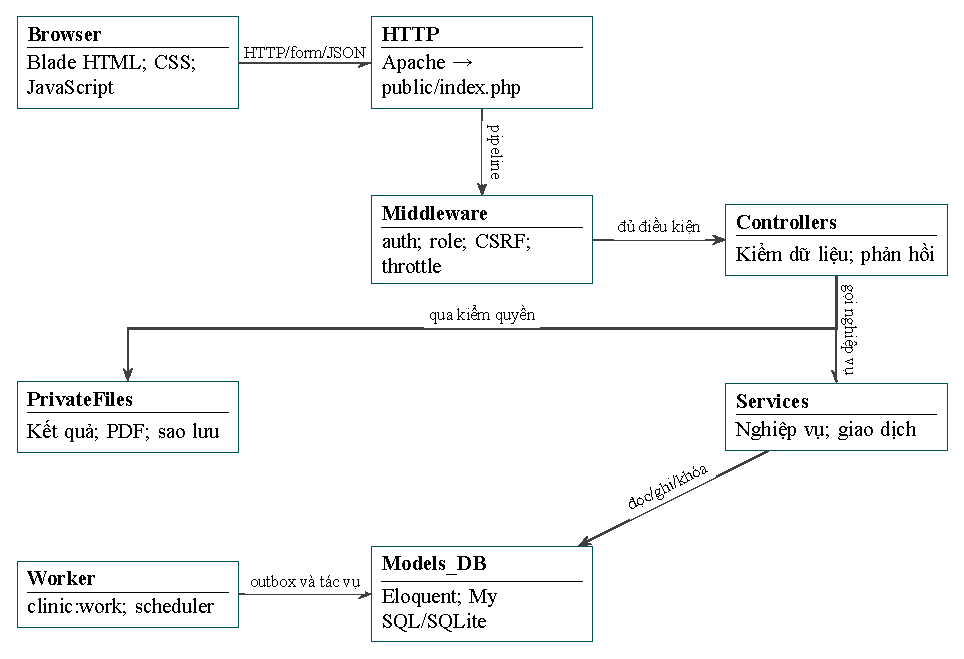
\includegraphics[width=1\textwidth,height=.61\textheight,keepaspectratio]{figures/diagrams/architecture.pdf}\captionof{figure}{Kiến trúc ứng dụng và phụ thuộc}\label{fig:architecture}\end{center}
Ứng dụng được tổ chức thành lớp giao diện, tiếp nhận yêu cầu, kiểm soát truy cập, xử lý nghiệp vụ và lưu trữ.\allowbreak{} Cơ sở dữ liệu lưu thông tin nghiệp vụ cùng hàng đợi thông báo.\allowbreak{} Tệp riêng được truy cập qua điểm tải có kiểm soát quyền.\allowbreak{} Các mũi tên thể hiện hướng xử lý và phụ thuộc chính giữa các thành phần.\allowbreak{}

\clearpage

\Needspace{6\baselineskip}\subsection{Triển khai bản Laragon trên Windows}
\begin{center}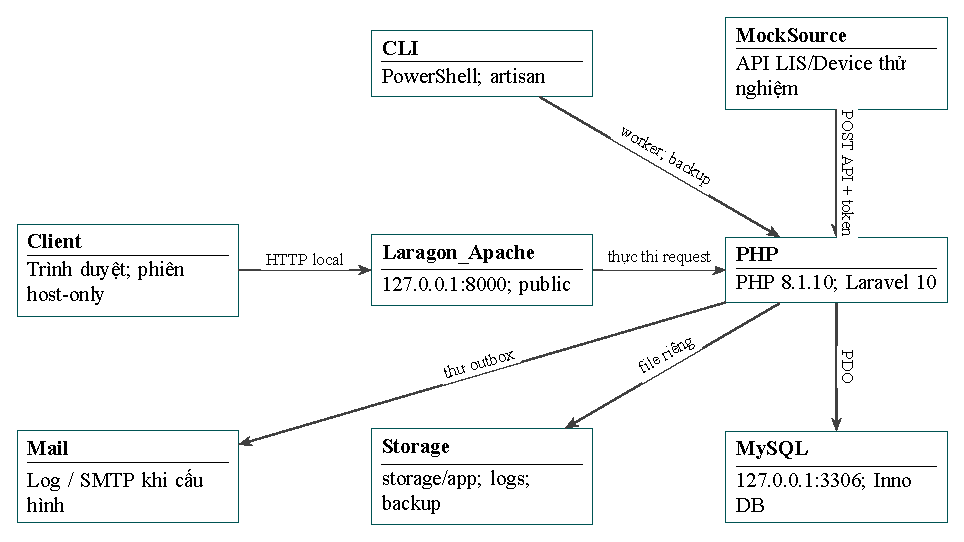
\includegraphics[width=1\textwidth,height=.61\textheight,keepaspectratio]{figures/diagrams/deployment.pdf}\captionof{figure}{Triển khai bản Laragon trên Windows}\label{fig:deployment}\end{center}
Sơ đồ mô tả môi trường học tập hiện tại.\allowbreak{} Khi triển khai ngoài máy local cần HTTPS và cấu hình hạ tầng riêng; không dùng sơ đồ này để khẳng định có phân cụm, dự phòng hoặc mail production.\allowbreak{} SQLite test tách khỏi My\allowbreak{}SQL vận hành.\allowbreak{}

\clearpage

\section{Thiết kế lớp và phụ thuộc}

\Needspace{6\baselineskip}\subsection{Lớp thiết kế phân hệ lịch}
\begin{center}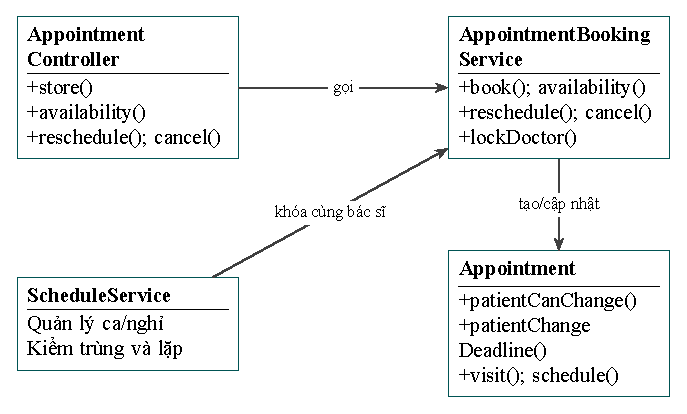
\includegraphics[width=1\textwidth,height=.61\textheight,keepaspectratio]{figures/diagrams/class_booking.pdf}\captionof{figure}{Lớp thiết kế phân hệ lịch}\label{fig:class_booking}\end{center}
Sơ đồ mô tả các lớp trọng tâm, thao tác và trách nhiệm của phân hệ.\allowbreak{} Dấu + biểu thị thao tác công khai.\allowbreak{} Các mũi tên thể hiện hướng sử dụng hoặc phụ thuộc giữa các lớp; dữ liệu lưu trữ được trình bày riêng trong lược đồ quan hệ và từ điển dữ liệu.\allowbreak{}

\clearpage

\Needspace{6\baselineskip}\subsection{Lớp thiết kế khám và kết quả}
\begin{center}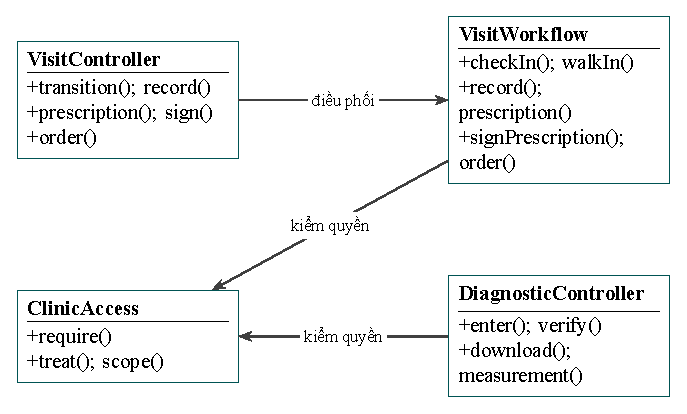
\includegraphics[width=1\textwidth,height=.61\textheight,keepaspectratio]{figures/diagrams/class_care.pdf}\captionof{figure}{Lớp thiết kế khám và kết quả}\label{fig:class_care}\end{center}
Sơ đồ mô tả các lớp trọng tâm, thao tác và trách nhiệm của phân hệ.\allowbreak{} Dấu + biểu thị thao tác công khai.\allowbreak{} Các mũi tên thể hiện hướng sử dụng hoặc phụ thuộc giữa các lớp; dữ liệu lưu trữ được trình bày riêng trong lược đồ quan hệ và từ điển dữ liệu.\allowbreak{}

\clearpage

\Needspace{6\baselineskip}\subsection{Lớp thiết kế tiền, kho và báo cáo}
\begin{center}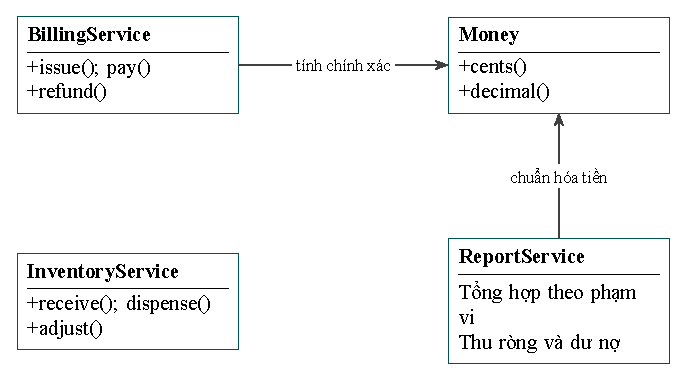
\includegraphics[width=1\textwidth,height=.61\textheight,keepaspectratio]{figures/diagrams/class_operations.pdf}\captionof{figure}{Lớp thiết kế tiền, kho và báo cáo}\label{fig:class_operations}\end{center}
Sơ đồ mô tả các lớp trọng tâm, thao tác và trách nhiệm của phân hệ.\allowbreak{} Dấu + biểu thị thao tác công khai.\allowbreak{} Các mũi tên thể hiện hướng sử dụng hoặc phụ thuộc giữa các lớp; dữ liệu lưu trữ được trình bày riêng trong lược đồ quan hệ và từ điển dữ liệu.\allowbreak{}

\clearpage

\Needspace{6\baselineskip}\subsection{Lớp thiết kế lịch nhân viên và lương}
\begin{center}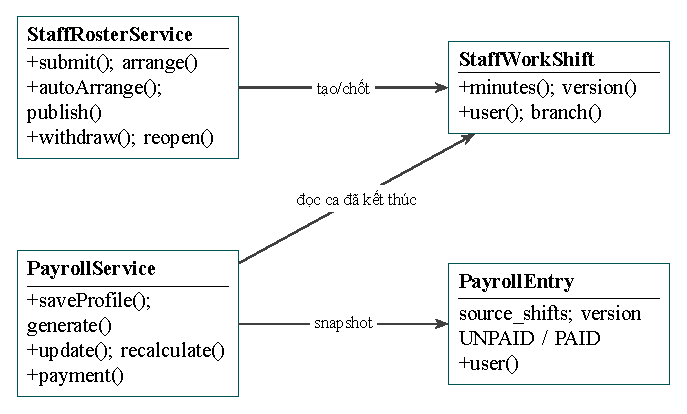
\includegraphics[width=1\textwidth,height=.61\textheight,keepaspectratio]{figures/diagrams/class_hr.pdf}\captionof{figure}{Lớp thiết kế lịch nhân viên và lương}\label{fig:class_hr}\end{center}
Sơ đồ mô tả các lớp trọng tâm, thao tác và trách nhiệm của phân hệ.\allowbreak{} Dấu + biểu thị thao tác công khai.\allowbreak{} Các mũi tên thể hiện hướng sử dụng hoặc phụ thuộc giữa các lớp; dữ liệu lưu trữ được trình bày riêng trong lược đồ quan hệ và từ điển dữ liệu.\allowbreak{}

\clearpage

\section{Tuần tự thiết kế các thao tác trọng yếu}

\Needspace{6\baselineskip}\subsection{Tuần tự thiết kế:\allowbreak{} đặt lịch}
\begin{center}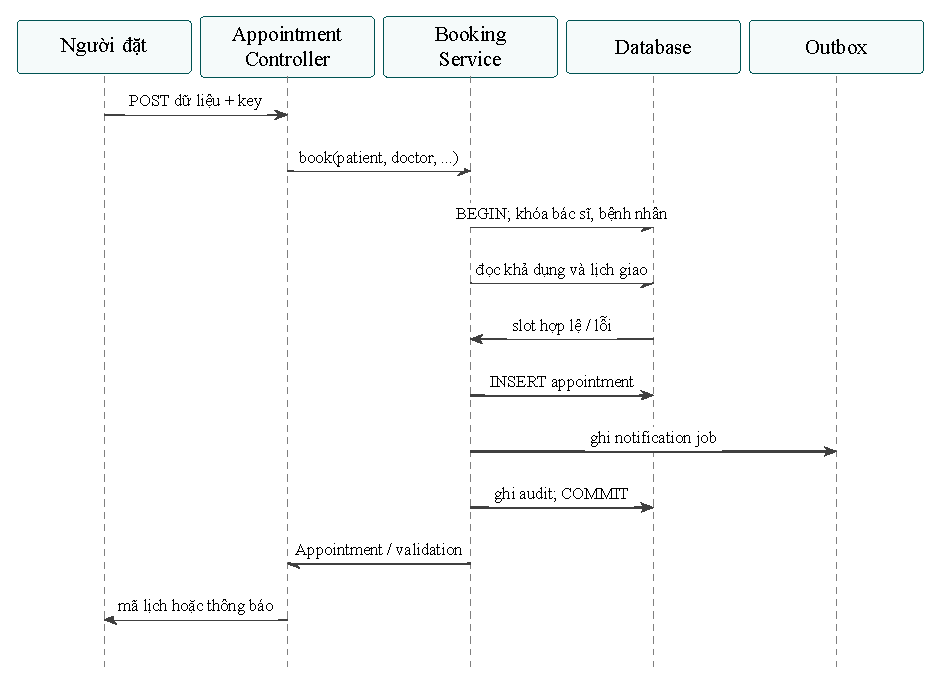
\includegraphics[width=1\textwidth,height=.61\textheight,keepaspectratio]{figures/diagrams/seq_book.pdf}\captionof{figure}{Tuần tự thiết kế:\allowbreak{} đặt lịch}\label{fig:seq_book}\end{center}
Giao dịch bao trùm kiểm tra cuối cùng và ghi dữ liệu.\allowbreak{} Nhánh cùng khóa trả lịch cũ khi thông tin khớp; khác nội dung là 409.\allowbreak{} Outbox trong sơ đồ là bảng cùng database, không phải dịch vụ email đang được gọi đồng bộ.\allowbreak{}

\clearpage

\Needspace{6\baselineskip}\subsection{Tuần tự thiết kế:\allowbreak{} tiếp nhận một lần}
\begin{center}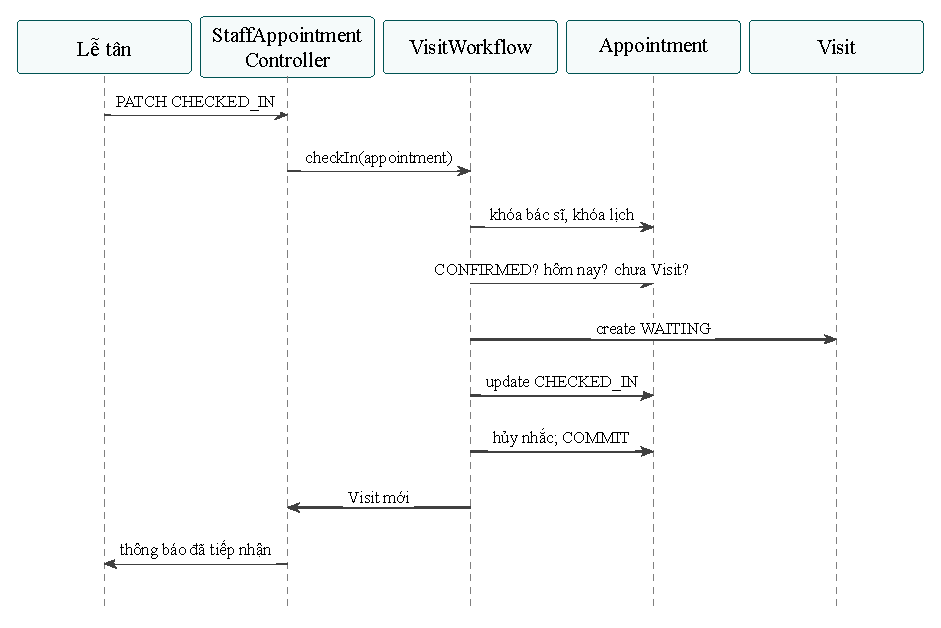
\includegraphics[width=1\textwidth,height=.61\textheight,keepaspectratio]{figures/diagrams/seq_checkin.pdf}\captionof{figure}{Tuần tự thiết kế:\allowbreak{} tiếp nhận một lần}\label{fig:seq_checkin}\end{center}
Visit được tạo cùng giao dịch đổi trạng thái lịch.\allowbreak{} Kiểm tra quyền được thực hiện theo cơ sở của bản lịch đã khóa.\allowbreak{} Việc bấm lặp không tạo lượt thứ hai; lỗi trạng thái web trở lại form còn JSON giữ mã lỗi phù hợp.\allowbreak{}

\clearpage

\Needspace{6\baselineskip}\subsection{Tuần tự thiết kế:\allowbreak{} thu tiền chống lặp}
\begin{center}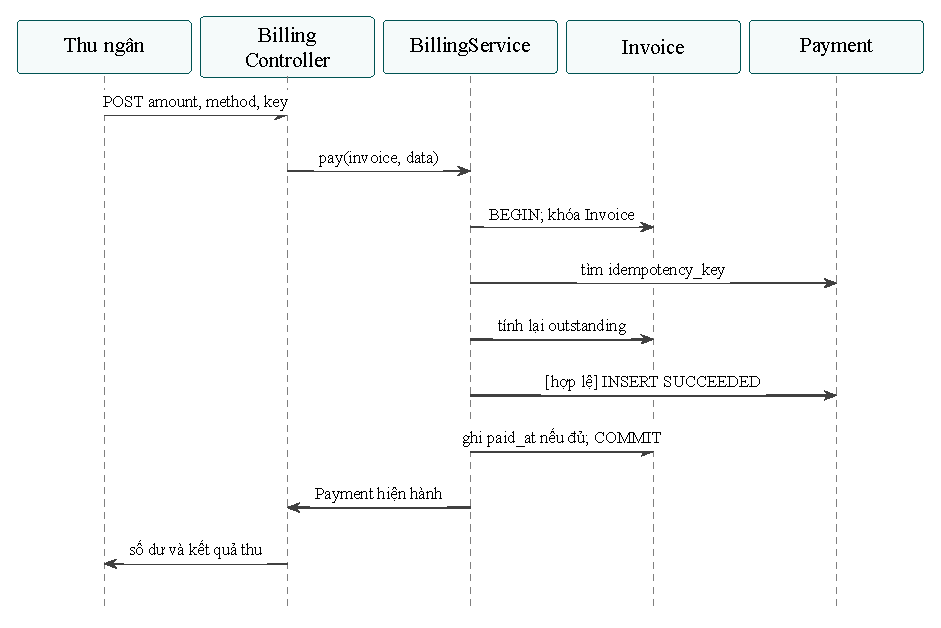
\includegraphics[width=1\textwidth,height=.61\textheight,keepaspectratio]{figures/diagrams/seq_payment.pdf}\captionof{figure}{Tuần tự thiết kế:\allowbreak{} thu tiền chống lặp}\label{fig:seq_payment}\end{center}
Nếu khóa đã tồn tại, máy chủ so invoice/\allowbreak{}amount/\allowbreak{}method/\allowbreak{}reference trước khi trả lại.\allowbreak{} Nếu chưa có, số tiền phải dương và không vượt số dư sau khóa.\allowbreak{} TRANSFER cần xác nhận; đây chưa là xác minh tự động từ ngân hàng.\allowbreak{}

\clearpage

\Needspace{6\baselineskip}\subsection{Tuần tự thiết kế:\allowbreak{} cấp thuốc theo lô}
\begin{center}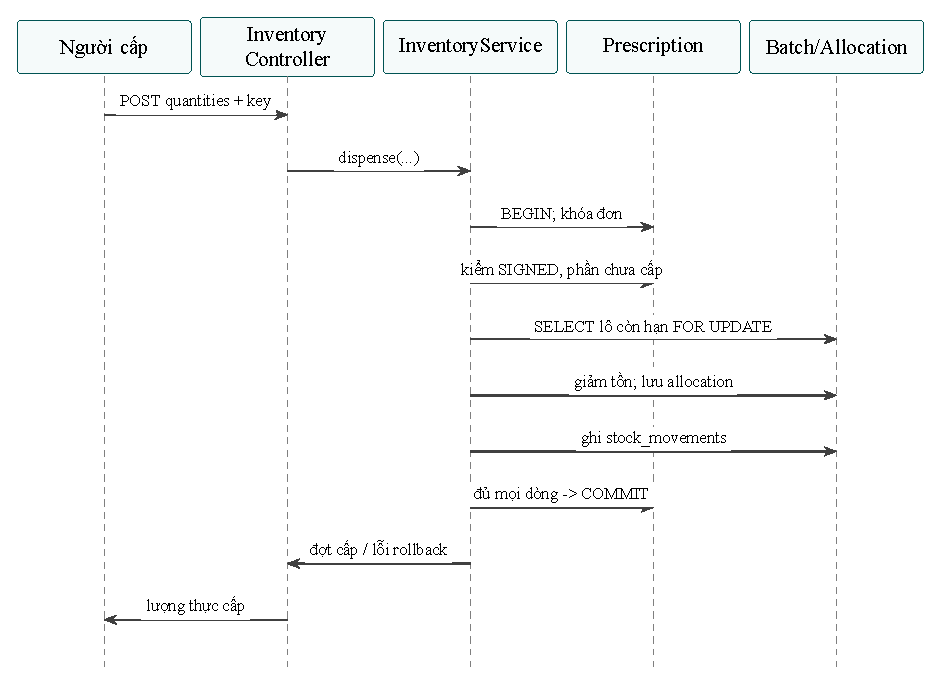
\includegraphics[width=1\textwidth,height=.61\textheight,keepaspectratio]{figures/diagrams/seq_fefo.pdf}\captionof{figure}{Tuần tự thiết kế:\allowbreak{} cấp thuốc theo lô}\label{fig:seq_fefo}\end{center}
Vòng lặp các lô thực hiện theo hạn dùng rồi ID.\allowbreak{} Nếu một dòng không đủ tồn, transaction rollback cả allocation và các lần giảm trước đó.\allowbreak{} Đơn đã ký là điều kiện cần, nhưng không đủ để bỏ kiểm cơ sở hay lượng đã cấp.\allowbreak{}

\clearpage

\Needspace{6\baselineskip}\subsection{Tuần tự thiết kế:\allowbreak{} lập bảng lương tháng}
\begin{center}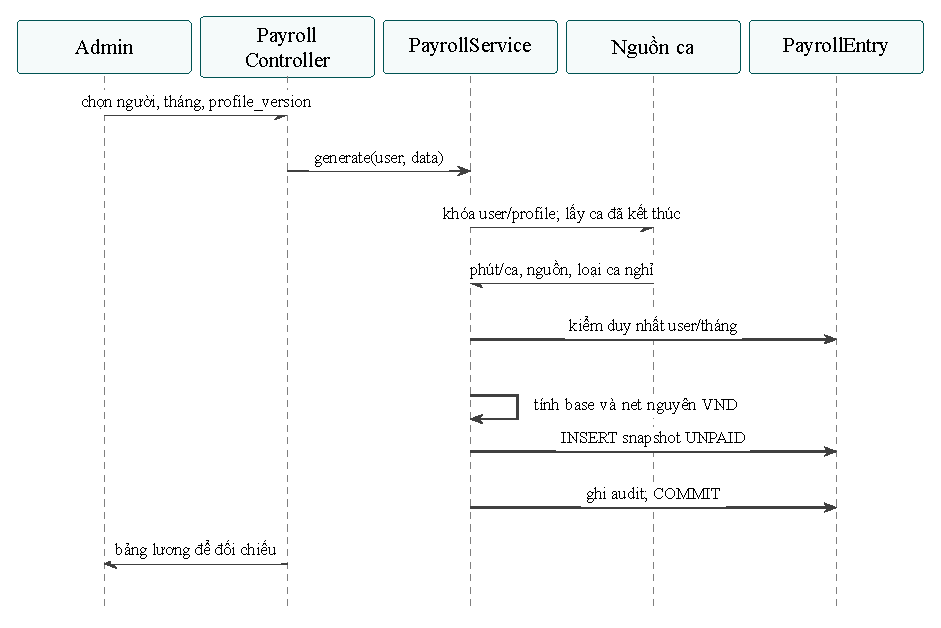
\includegraphics[width=1\textwidth,height=.61\textheight,keepaspectratio]{figures/diagrams/seq_payroll.pdf}\captionof{figure}{Tuần tự thiết kế:\allowbreak{} lập bảng lương tháng}\label{fig:seq_payroll}\end{center}
Nguồn ca là lịch đã kết thúc, chưa chứng minh chấm công.\allowbreak{} Bảng tháng ghi lại nguồn để admin đối chiếu.\allowbreak{} Chỉ admin được lập/\allowbreak{}chỉnh; nhân viên dùng đường đọc riêng được giới hạn sở hữu.\allowbreak{}

\clearpage

\Needspace{6\baselineskip}\subsection{Tuần tự thiết kế:\allowbreak{} bác sĩ nhận chuyển ca}
\begin{center}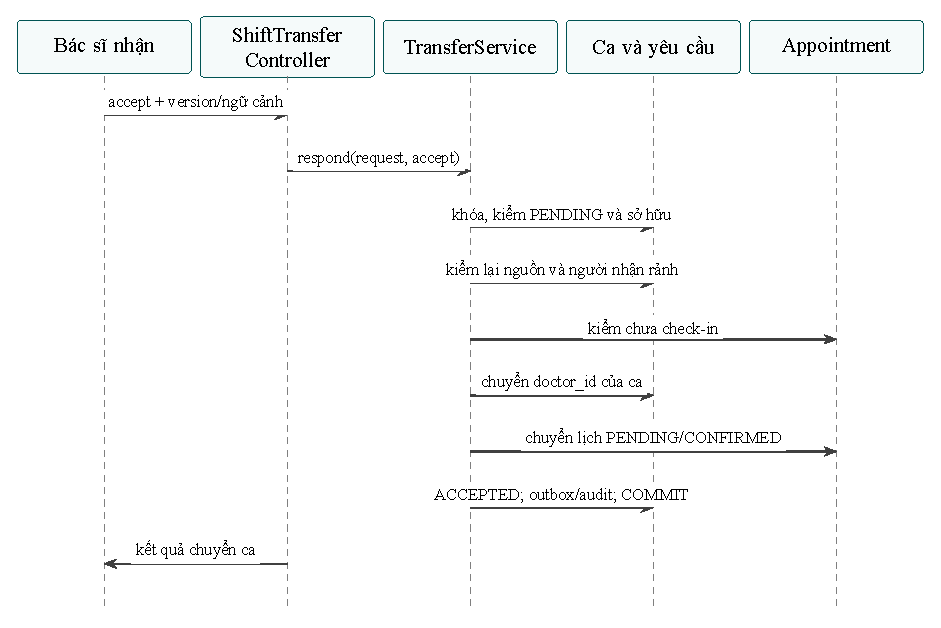
\includegraphics[width=1\textwidth,height=.61\textheight,keepaspectratio]{figures/diagrams/seq_transfer.pdf}\captionof{figure}{Tuần tự thiết kế:\allowbreak{} bác sĩ nhận chuyển ca}\label{fig:seq_transfer}\end{center}
Người nhận có thể rảnh ở lúc gửi nhưng bận ở lúc chấp nhận; dịch vụ kiểm lại bên trong transaction.\allowbreak{} Ca và lịch còn hiệu lực phải đổi cùng nhau.\allowbreak{} Lịch hủy/\allowbreak{}vắng và dữ liệu khám lịch sử không được thay người phụ trách theo thao tác này.\allowbreak{}

\clearpage

\section{Thiết kế lược đồ quan hệ}

\Needspace{6\baselineskip}\subsection{Lược đồ quan hệ:\allowbreak{} danh tính và phân công}
\begin{center}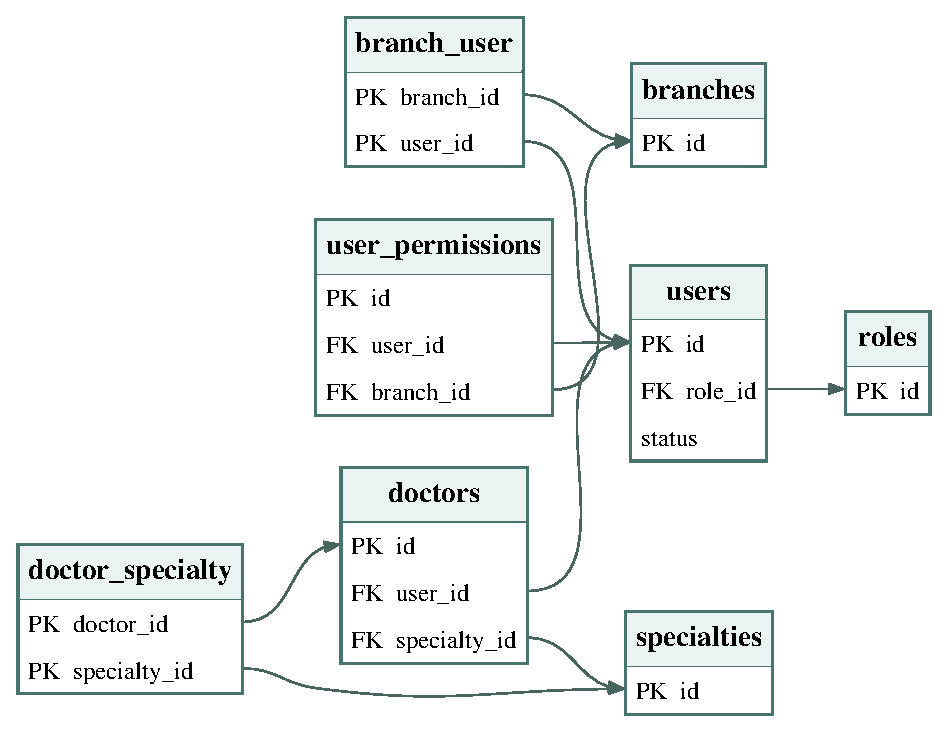
\includegraphics[width=1\textwidth,height=.61\textheight,keepaspectratio]{figures/diagrams/erd_identity.pdf}\captionof{figure}{Lược đồ quan hệ:\allowbreak{} danh tính và phân công}\label{fig:erd_identity}\end{center}
Đường nối xuất phát ở dòng FK và đi tới khóa được tham chiếu.\allowbreak{} Hình chỉ chọn các cột và liên kết trong nhóm; khóa actor và liên kết ra nhóm khác được lược bớt.\allowbreak{} Bội số chính xác được suy từ nullable và chỉ mục UNIQUE trong từ điển dữ liệu.\allowbreak{} Mũi tên biểu thị tham chiếu dữ liệu, không phải kế thừa.\allowbreak{}

\clearpage

\Needspace{6\baselineskip}\subsection{Lược đồ quan hệ:\allowbreak{} ca khám và lịch hẹn}
\begin{center}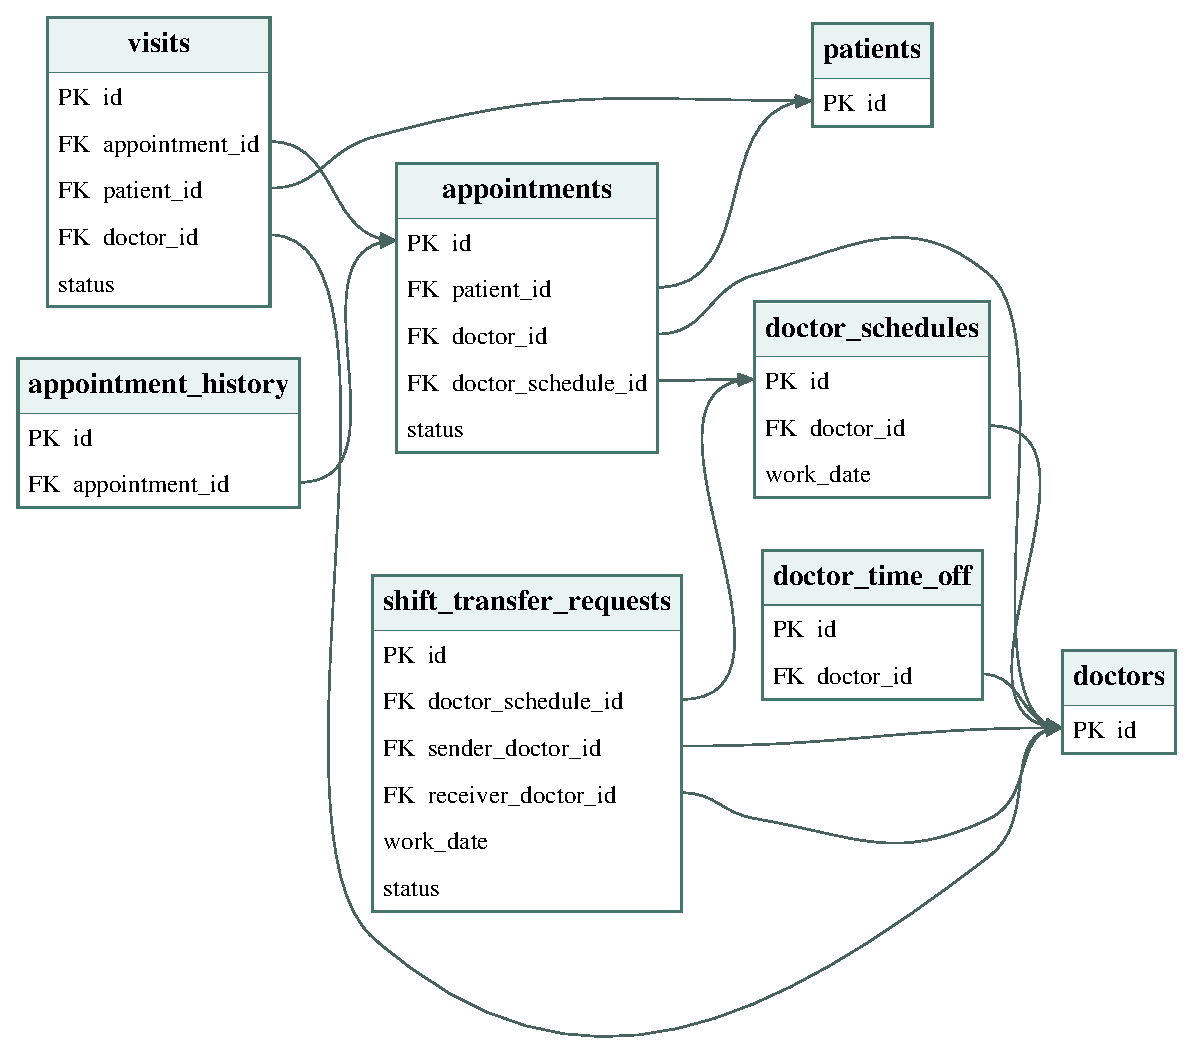
\includegraphics[width=1\textwidth,height=.61\textheight,keepaspectratio]{figures/diagrams/erd_booking.pdf}\captionof{figure}{Lược đồ quan hệ:\allowbreak{} ca khám và lịch hẹn}\label{fig:erd_booking}\end{center}
Đường nối xuất phát ở dòng FK và đi tới khóa được tham chiếu.\allowbreak{} Hình chỉ chọn các cột và liên kết trong nhóm; khóa actor và liên kết ra nhóm khác được lược bớt.\allowbreak{} Bội số chính xác được suy từ nullable và chỉ mục UNIQUE trong từ điển dữ liệu.\allowbreak{} Mũi tên biểu thị tham chiếu dữ liệu, không phải kế thừa.\allowbreak{}

\clearpage

\Needspace{6\baselineskip}\subsection{Lược đồ quan hệ:\allowbreak{} hồ sơ và đơn thuốc}
\begin{center}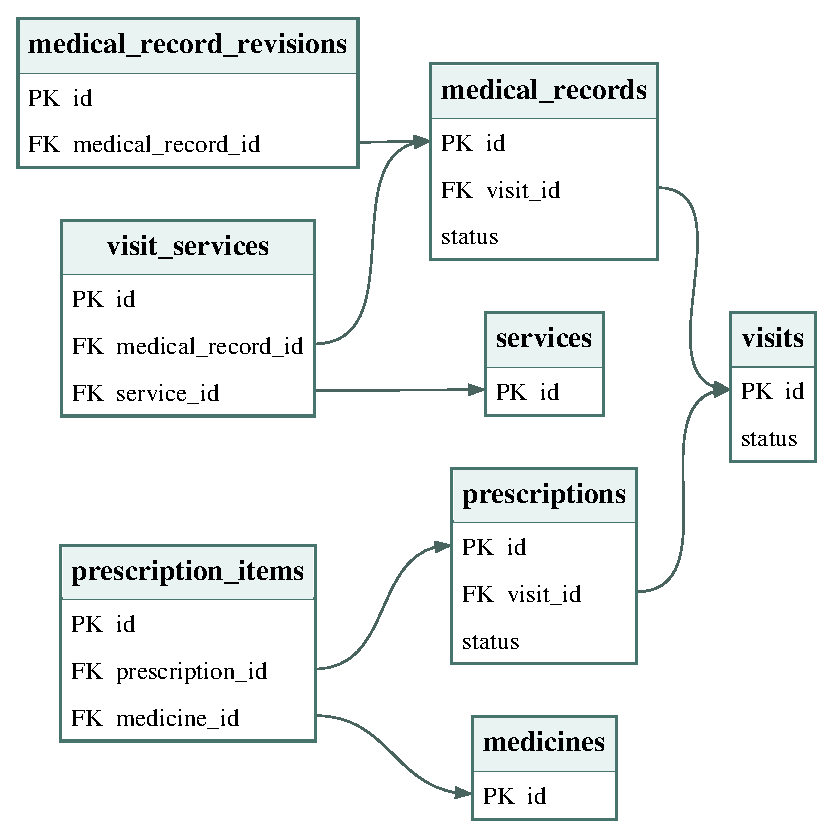
\includegraphics[width=1\textwidth,height=.61\textheight,keepaspectratio]{figures/diagrams/erd_clinical.pdf}\captionof{figure}{Lược đồ quan hệ:\allowbreak{} hồ sơ và đơn thuốc}\label{fig:erd_clinical}\end{center}
Đường nối xuất phát ở dòng FK và đi tới khóa được tham chiếu.\allowbreak{} Hình chỉ chọn các cột và liên kết trong nhóm; khóa actor và liên kết ra nhóm khác được lược bớt.\allowbreak{} Bội số chính xác được suy từ nullable và chỉ mục UNIQUE trong từ điển dữ liệu.\allowbreak{} Mũi tên biểu thị tham chiếu dữ liệu, không phải kế thừa.\allowbreak{}

\clearpage

\Needspace{6\baselineskip}\subsection{Lược đồ quan hệ:\allowbreak{} chỉ định, kết quả và tái khám}
\begin{center}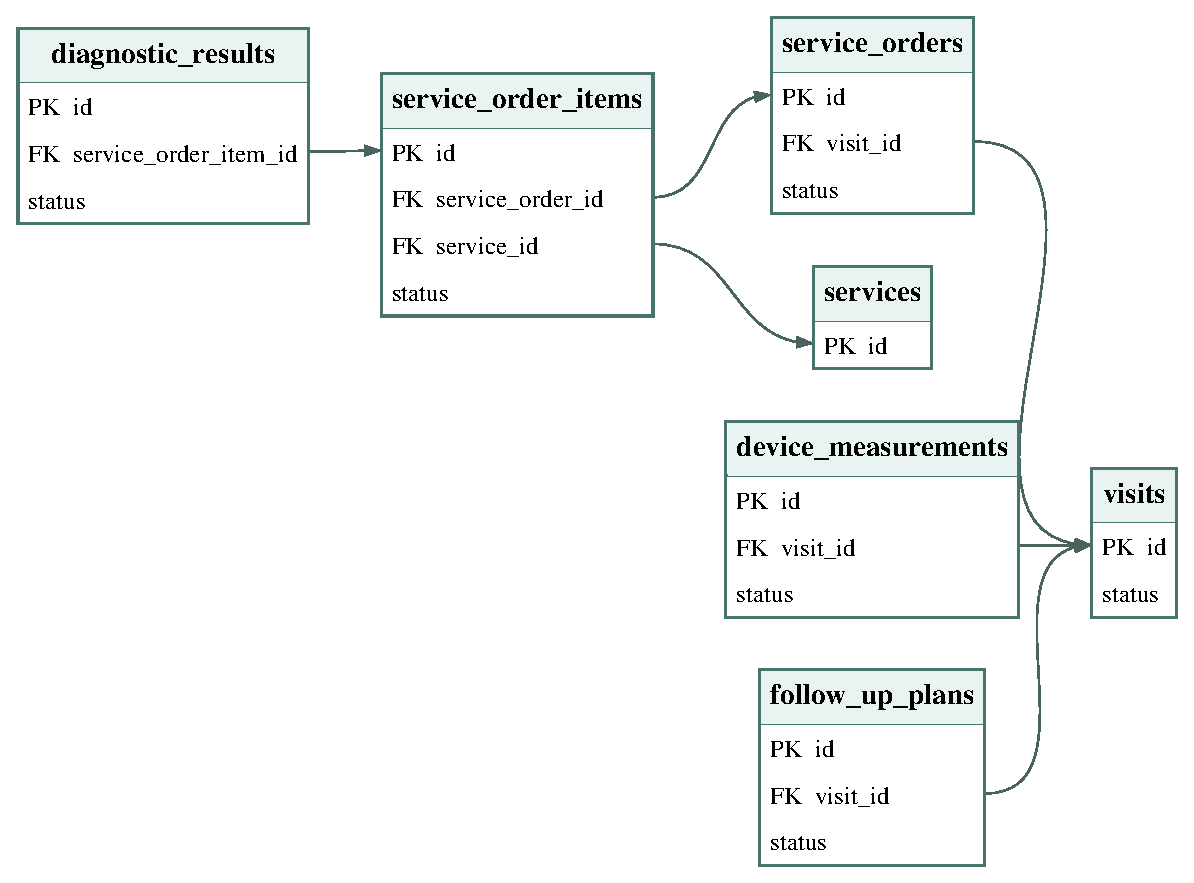
\includegraphics[width=1\textwidth,height=.61\textheight,keepaspectratio]{figures/diagrams/erd_diagnostic.pdf}\captionof{figure}{Lược đồ quan hệ:\allowbreak{} chỉ định, kết quả và tái khám}\label{fig:erd_diagnostic}\end{center}
Đường nối xuất phát ở dòng FK và đi tới khóa được tham chiếu.\allowbreak{} Hình chỉ chọn các cột và liên kết trong nhóm; khóa actor và liên kết ra nhóm khác được lược bớt.\allowbreak{} Bội số chính xác được suy từ nullable và chỉ mục UNIQUE trong từ điển dữ liệu.\allowbreak{} Mũi tên biểu thị tham chiếu dữ liệu, không phải kế thừa.\allowbreak{}

\clearpage

\Needspace{6\baselineskip}\subsection{Lược đồ quan hệ:\allowbreak{} hóa đơn và dòng tiền}
\begin{center}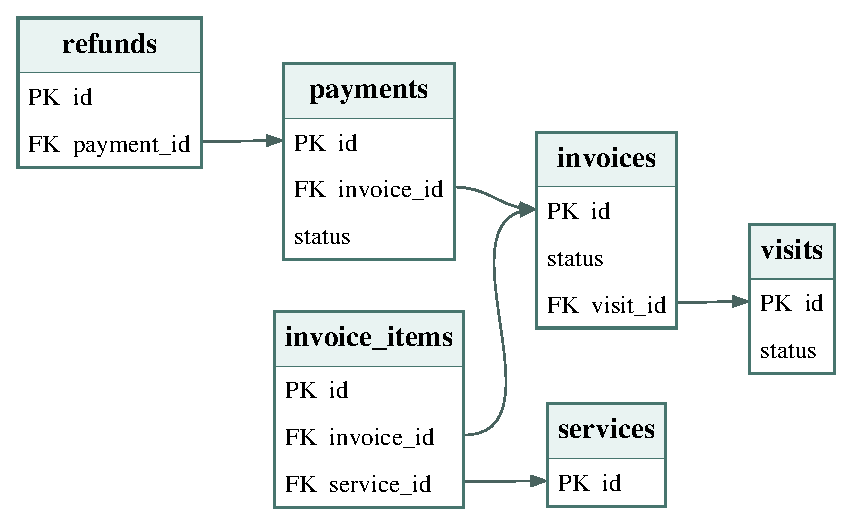
\includegraphics[width=1\textwidth,height=.61\textheight,keepaspectratio]{figures/diagrams/erd_finance.pdf}\captionof{figure}{Lược đồ quan hệ:\allowbreak{} hóa đơn và dòng tiền}\label{fig:erd_finance}\end{center}
Đường nối xuất phát ở dòng FK và đi tới khóa được tham chiếu.\allowbreak{} Hình chỉ chọn các cột và liên kết trong nhóm; khóa actor và liên kết ra nhóm khác được lược bớt.\allowbreak{} Bội số chính xác được suy từ nullable và chỉ mục UNIQUE trong từ điển dữ liệu.\allowbreak{} Mũi tên biểu thị tham chiếu dữ liệu, không phải kế thừa.\allowbreak{}

\clearpage

\Needspace{6\baselineskip}\subsection{Lược đồ quan hệ:\allowbreak{} kho và cấp phát theo lô}
\begin{center}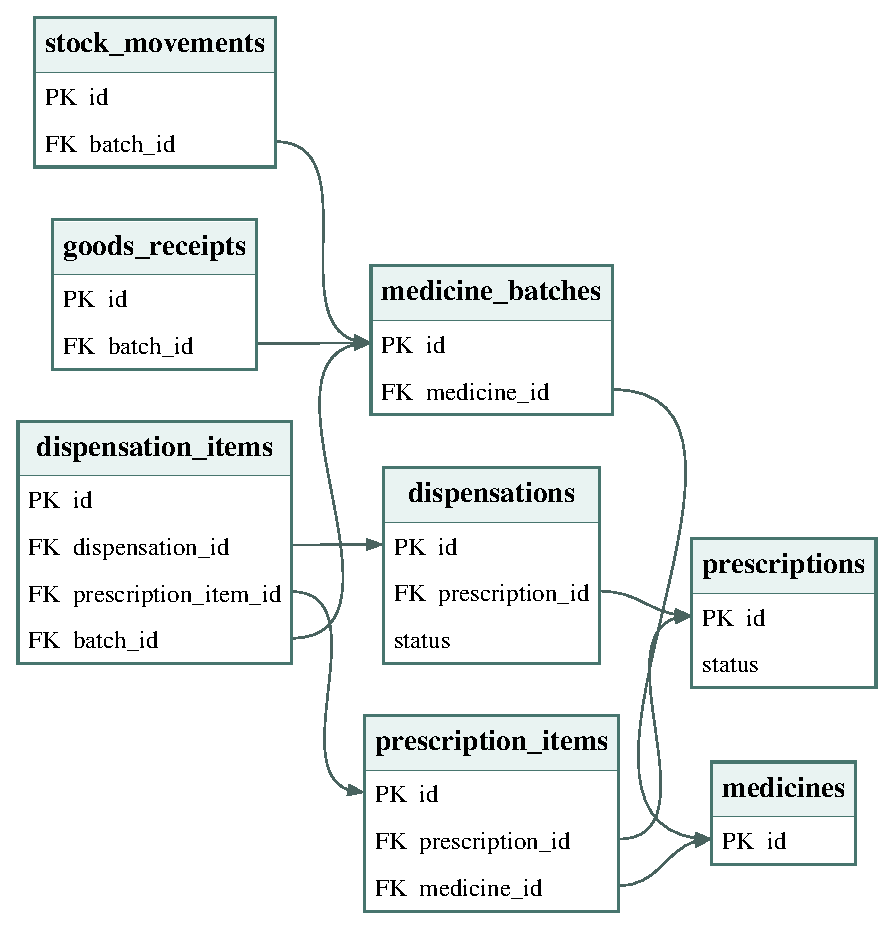
\includegraphics[width=1\textwidth,height=.61\textheight,keepaspectratio]{figures/diagrams/erd_inventory.pdf}\captionof{figure}{Lược đồ quan hệ:\allowbreak{} kho và cấp phát theo lô}\label{fig:erd_inventory}\end{center}
Đường nối xuất phát ở dòng FK và đi tới khóa được tham chiếu.\allowbreak{} Hình chỉ chọn các cột và liên kết trong nhóm; khóa actor và liên kết ra nhóm khác được lược bớt.\allowbreak{} Bội số chính xác được suy từ nullable và chỉ mục UNIQUE trong từ điển dữ liệu.\allowbreak{} Mũi tên biểu thị tham chiếu dữ liệu, không phải kế thừa.\allowbreak{}

\clearpage

\Needspace{6\baselineskip}\subsection{Lược đồ quan hệ:\allowbreak{} nhân viên và bảng lương}
\begin{center}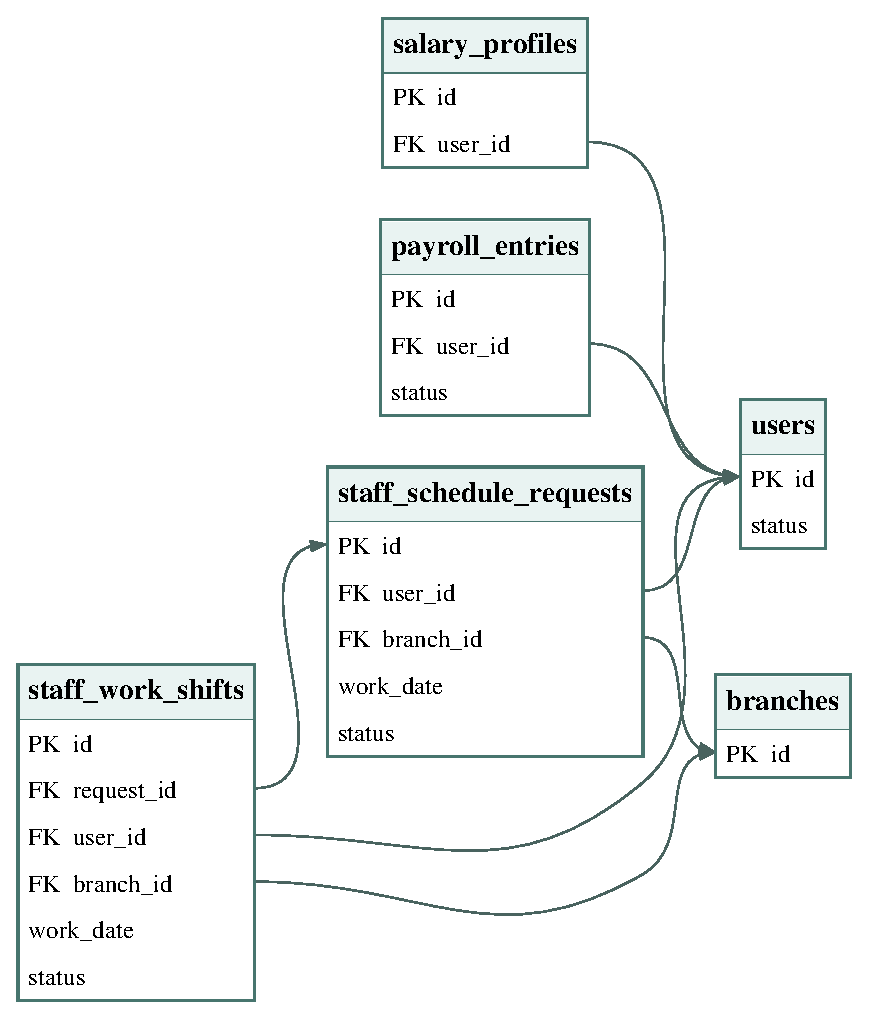
\includegraphics[width=1\textwidth,height=.61\textheight,keepaspectratio]{figures/diagrams/erd_workforce.pdf}\captionof{figure}{Lược đồ quan hệ:\allowbreak{} nhân viên và bảng lương}\label{fig:erd_workforce}\end{center}
Đường nối xuất phát ở dòng FK và đi tới khóa được tham chiếu.\allowbreak{} Hình chỉ chọn các cột và liên kết trong nhóm; khóa actor và liên kết ra nhóm khác được lược bớt.\allowbreak{} Bội số chính xác được suy từ nullable và chỉ mục UNIQUE trong từ điển dữ liệu.\allowbreak{} Mũi tên biểu thị tham chiếu dữ liệu, không phải kế thừa.\allowbreak{}

\clearpage

\Needspace{6\baselineskip}\subsection{Lược đồ quan hệ:\allowbreak{} tích hợp và thông báo}
\begin{center}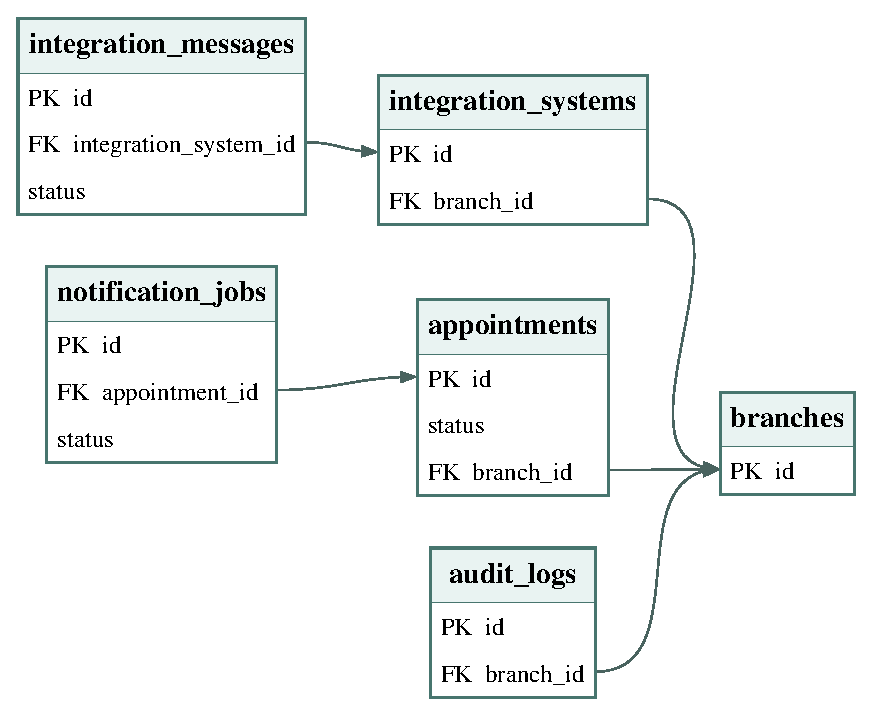
\includegraphics[width=1\textwidth,height=.61\textheight,keepaspectratio]{figures/diagrams/erd_integration.pdf}\captionof{figure}{Lược đồ quan hệ:\allowbreak{} tích hợp và thông báo}\label{fig:erd_integration}\end{center}
Đường nối xuất phát ở dòng FK và đi tới khóa được tham chiếu.\allowbreak{} Hình chỉ chọn các cột và liên kết trong nhóm; khóa actor và liên kết ra nhóm khác được lược bớt.\allowbreak{} Bội số chính xác được suy từ nullable và chỉ mục UNIQUE trong từ điển dữ liệu.\allowbreak{} Mũi tên biểu thị tham chiếu dữ liệu, không phải kế thừa.\allowbreak{}

\clearpage

\section{Thiết kế lưu trữ và từ điển dữ liệu}
Phụ lục A trình bày thiết kế chi tiết của 52 bảng, gồm bảng nghiệp vụ và bảng nền tảng.\allowbreak{} Mỗi bảng được mô tả theo mục đích, thuộc tính, kiểu dữ liệu, tính bắt buộc, khóa và chỉ mục.\allowbreak{} Phần tương thích dữ liệu cũ được phân biệt với cấu trúc dùng cho các quy trình mới.\allowbreak{}

My\allowbreak{}SQL là cơ sở dữ liệu triển khai trên Laragon; SQLite được dùng cho kiểm thử cô lập.\allowbreak{} Các khóa ngoại bảo vệ quan hệ tham chiếu, chỉ mục duy nhất bảo vệ định danh và quan hệ một-một.\allowbreak{} Những ràng buộc liên quan tổng tiền, tổng số lượng và khoảng thời gian còn được kiểm tra trong giao dịch của lớp nghiệp vụ.\allowbreak{}


{\small\setlength{\tabcolsep}{3pt}\renewcommand{\arraystretch}{1.12}
\begin{longtable}{@{}L{\dimexpr 0.25\textwidth-1.5pt\relax} L{\dimexpr 0.75\textwidth-4.5pt\relax}@{}}
\caption{Tóm tắt kiểm soát toàn vẹn}\\
\toprule
\textbf{Nhóm dữ liệu} & \textbf{Chiến lược toàn vẹn}\\\midrule
\endfirsthead
\toprule
\textbf{Nhóm dữ liệu} & \textbf{Chiến lược toàn vẹn}\\\midrule
\endhead
\bottomrule\endlastfoot
Danh tính/\allowbreak{}cơ sở & UNIQUE email, mã; FK và phân công; kiểm role/\allowbreak{}permission trong ứng dụng.\allowbreak{}\\[3pt]
Lịch/\allowbreak{}ca & Khóa bác sĩ, bệnh nhân; kiểm giao khoảng, trạng thái và lịch nghỉ trong transaction.\allowbreak{}\\[3pt]
Khám/\allowbreak{}kết quả & Visit làm gốc; version hồ sơ; snapshot revision; quyền ký/\allowbreak{}duyệt.\allowbreak{}\\[3pt]
Tài chính & Khóa hóa đơn; snapshot dòng; UNIQUE idempotency; hoàn theo Payment.\allowbreak{}\\[3pt]
Kho & Khóa đơn/\allowbreak{}lô; giảm có điều kiện; chứng từ và allocation cùng transaction.\allowbreak{}\\[3pt]
Nhân sự/\allowbreak{}lương & Fingerprint chốt ca, version bảng lương, UNIQUE user/\allowbreak{}tháng; nguồn ca chụp JSON.\allowbreak{}\\[3pt]
\end{longtable}}
